\documentclass[a4paper,11pt]{report}
\usepackage{fullpage}
\usepackage{comment}
\usepackage[colorinlistoftodos]{todonotes}
%\usepackage{cite}
\usepackage{lmodern}
\usepackage[T1]{fontenc}
\usepackage{textcomp}
\usepackage{xcolor,graphicx} % Future use
\usepackage{caption}
\usepackage{hyperref}
\usepackage[all]{hypcap}
\hypersetup{colorlinks=false, pdfborder={0 0 0}}
\usepackage{multirow}
\usepackage{amsmath}
\usepackage{tikz}
\usepackage{tkz-euclide}
\usepackage{pgfplots}
\pgfplotsset{compat=1.9}
\usetkzobj{all}
\usetikzlibrary{calc,backgrounds,positioning}
\usetikzlibrary{shapes,arrows}
\usepackage[numbers]{natbib}
\usepackage{amsfonts}
\newcommand{\tickYes}{\checkmark}
\usepackage{pifont}
\newcommand{\tickNo}{\hspace{1pt}\ding{55}}
\newcommand{\note}[1]{}
\usepackage{listings}
\usepackage{subcaption}
\usepackage{tkz-euclide}
\usepackage{float}
\usepackage{subcaption}
\usepackage[utf8]{inputenc}
\usepackage{algorithm}
\usepackage{algpseudocode}

\newcommand*\Let[2]{\State #1 $\gets$ #2}

\widowpenalty 10000
\clubpenalty 10000

\newcolumntype{x}[1]{%
>{\raggedleft\hspace{0pt}}p{#1}}%

% http://www.tex.ac.uk/ctan/macros/latex/contrib/todonotes/todonotes.pdf

\usepackage{blindtext}
\parskip=12pt % adds vertical space between paragraphs

\begin{document}
\pagenumbering{roman}
\pagestyle{plain} % only page numbers at the bottom

\listoftodos

\thispagestyle{empty}
\title{Interactive point cloud segmentation}
\author{Rickert Mulder}
\maketitle

% \tableofcontents
% \listoffigures
\listofalgorithms

% \newpage
% \chapter*{Acknowledgements}
% I'd like to thank my legs for always suporting me, my arms of always being on my side, and my fingers beacuse I can always count on them.
% \addcontentsline{toc}{section}{Acknowledgements}

% \listoftables


% \begin{abstract}
% Point cloud cleaning is an important but time consuming step in a 3d reconstruction pipeline. In this thesis, we investigate how computer vision an machine learning techniques can be used to expedite this task. Early vision algorithms are investigated and later combined with higher level techniques. We finally show how random forest can be interactively trained to find arbitrary objects which reduced the time subjects require to complete a cleaning task.
% \end{abstract}

% \clearpage
\pagenumbering{arabic}
%\chapter{Introduction}

\section{Research question}


\section{System overview}


\section{Outline}
Explain what is discussed in the following chapters


% Motivation & research question
% Ethics
% Background we need to know
%!TEX root = thesis.tex
\chapter{Background} \label{ch2}

In order to expedited the segmentation of laser range scans its important to both understand the problem domain as well as constrain the problem. We start this chapter by examining laser range scanning technology and how it is employed in the context cultural heritage domain.

\section{Range scanners}
	
There is an enormous variety of range scanners. Time of flight scanners are generally used in the cultural heritage domain because of their long range (up to kilometers). Time of flight scanners work by sending out a laser pulses that reflect of objects and is then recorded by a sensor at the source. The time it takes to the pulse to return, along with the angle at which the pulse was fired, is used to determine the position of a point on a surface. There is more measurement error (millimeters) along the direction of the laser than the other two axis. This is due to measurement inaccuracies when timing the laser's travel time. Triangulation scanners are more accurate along the direction of the beam (tens of micrometers), but they have a shorter range compared to time of flight scanners. This makes them less popular when people try minimize the number of scans required to capture a site. (Other types of range scanners include structure from motion and structured light.)

Time of flight scanners can be set to sample at different resolutions. Low resolution scans (10 000 points) may take seconds while higher resolution scans (millions of points) may take minutes depending on the model. All scanners return the X,Y and Z coordinates per sample. Most also return an intensity value of the reflected light. More expensive scanners are also mounted with a camera that associates RGB values with every sample. This makes it easier to texture (texture) the final model. Measuring the orientation and GPS position of the scanner is another optional feature that can ease registration process (discussed later).

(Mention Averaged pixel on edges for time of flight)
(Mention multiple sample pulse scanners)
(Mention non uniform point density somewhere? too obvious?)
(Mention scanner resolution increasing over time?)

\section{3D reconstruction pipeline}
Some processing is required in order to create a 3d model from a collection of laser range scans. Unwanted objects need to be removed or cleaned. Holes created by removals and occlusions need to be filled. The scans need to registered. Registration is the process of aligning all the scans on a common coordinate system (mention Iterative closest points?).Then the registered point sets have to turned into a surface model. This is also called meshing. Finally the model has to be textured. RGB data from the scanner can be used if it available. Alternatively photos from the site has to be mapped to the model. The second approach is somewhat more time consuming.

The cleaning step can be omitted but the quality of the model will be affected. Objects such as trees or grass do not always mesh nicely, and floating bits of people as they walk around may not be aesthetically pleasing. Hole filling is also not strictly necessary. It can even be argued that it compromises the integrity of the historical record as the filled area would be fabricated.

The first 3 step also do not have to happen in order. It is often the case that hole filling, cleaning and registration tasks are interspersed. Cleaning may be detrimental to the reregistration process as useful correspondences may be removed. Cleaning scans after registration can however be problematic. If the scans have been merged into a single point cloud, loading the scan into main memory may not be an option on some programs. One also loses the 2d grid structure of the scan after merging. The scan's grid allows one to interpret the scan as a 2d image which may be easier to clean.


\section{Point cloud cleaning}
	Focused specifically on the task of point cloud cleaning in heritage scenes

	\subsection{Problem}
	Characterize heritage scenes
	\begin{itemize}
		\item Large scans
		\item many scans
		\item Non uniform density
		\item Large point sets
		\item Hard to distinguish trees from walls
	\end{itemize}

	\subsection{Existing systems}
		\begin{itemize}
			\item Z\&Y
			\item Cyclone
			\item Pointools
			\item Meshlab
			\item VR Mesh Studio
			\item Carlson Pointcloud
			\item 3D Reshaper
			\item Terrascan
		\end{itemize}

	\subsection{Evaluation of existing systems}
	We should look at existing systems in terms of a testing framework
	Evaluate their tools
	Evaluate user interface
	\begin{itemize}
		\item navigation: camera vs object move
		\item tool set (what tools are available)
		\item license
		\item 2d/3d editing
		\item extensibility (why did I not use it)
	\end{itemize}


\section{Previous work}
Point cloud cleaning is a interactive segmentation problem. Segmentation is by no means a new problem.

\subsection{Taxonomy}
\begin{itemize}
	\item Interactive/Automated
	\item Information: 2D/2.5D/3D/nD, color, multi-sample, intensity
	\item Resolution: High, Medium, Low
	\item Features: Texture, FPFH, Normals, ...
	\item Target: trees, ground, walls, people, generic
	\item Parameters: Low, Medium, High
\end{itemize}


\subsection{Image segmentation}
	Scans are simply a depth maps so 2D image techniques should be investigated
	\subsection{Image gradients}
	\subsection{Edge detection}
	\subsection{Blob extraction}
	\subsection{Contour extraction}

\subsection{Laser scan segmentation}
	\subsection{Point features}
		\subsubsection{Normals}
			Basic building block for other features
			\begin{itemize}
			\item Ways of performing normal estimation
			\item Neighbour search
				\begin{itemize}
				\item KD Trees
				\item Scan grid
				\end{itemize}
			\item Cost vs Quality
			\item Dealing with noise
			\item Used with machine learning algorithms
			\end{itemize}
				
		\subsubsection{Fast point feature histograms (FPFH)}
			\begin{itemize}
			\item Good discrimination for primitive geometric objects
			\item Costly to calculate
			\end{itemize}
			
		\subsubsection{Principle components}
			\begin{itemize}					
			\item Good for finding edges and planes
			\item Solves part of the inverse problem
			\end{itemize}
			

	\subsection{Region growing}
		\begin{itemize}
		\item Grow neighbourhood from seed point
		\item Add neighbour if it satisfies some similarity criteria
		\item Point feature can be used to determine similarity
		\end{itemize}

	\subsection{K-means clustering}
		Problems with non uniform density

	\subsection{Graph cuts}
		\begin{itemize}
		\item Binary classification
		\item Encode point similarity edges
		\item Shown to work well with arbitrary objects
		\item Results are parameter depended
		\end{itemize}

	\subsection{Machine learning}
		\begin{itemize}
		\item Used in navigation \& aerial scans
		\item Support vector machines
		\item Markov models
		\item Conditional random fields
		\item Requires training
		\end{itemize}
		
	% \subsection{Evaluation of literature}
	% 	\begin{itemize}
	% 	\item FPFH seems to discriminate well for primitive geometry. Might be a useful feature to use in tree classification.
	% 	\item Machine learning has been used to classify vegetation. It however requires training and classified datasets are rare. Possibility to train a classifier on the on scans in the application. Unpredictable accuracy.
	% 	\item Graph cuts have been shown be effective for automated object classification. Augmented with more edge information accuracy may be improved with minimal user interaction.
	% 	\end{itemize}

\section{Evaluation techniques}
\begin{itemize}
	\item What was used in previous work and would it be suitable in this instance?
\end{itemize}
	
% \section{User interaction}
% 	\begin{itemize}
% 		\item Level of interactivity expected?
% 		\item Characteristics of interfaces?
% 		\item Basic expected functionality?
% 		\item Suitable evaluation techniques
% 	\end{itemize}
		

\section{Conclusion}
%What do I conclude from all this and lead into the next chapter.		


%\chapter{Framework} \label{chapter:framework}
Point cloud cleaning is an intensive interactive task. Improved segmentation techniques can therefore not be created without considering the user interface that facilitates them. A bad interface can negate any gains to be had from better tools. An interface that is effective and easy to use is therefore a prerequisite for a faster segmentation process.

In \autoref{ch:background} it was argued that in order for a user to be effective, i.e. achieve a predetermined level of accuracy, techniques with a small area of influence are required in addition to techniques with large areas of influence. For example, a polygon selection tool can select a large area but can lack accuracy. In order to achieve a good level of accuracy a brush tool that has a small area of influence is needed to correct mislabeled points within the larger selection achieved by the lasso tool. It is clear that proprietary systems provide a larger range of tools when compared to open source alternatives. Proprietary tools also tend to be more user friendly. It would thus be preferable to use a proprietary system as a base for testing new segmentation techniques. Unfortunately, due to their closed sourced nature, we are forced to either extend an open source system or create one.

Allowing a user to undo an action or return to a previous state is an important usability heuristic \cite{Nielsen2005}. The importance of undo to user productivity was reiterated in informal talks with users of Meshlab in the heritage domain. Adding undo functionality to Meshlab or Cloud Compare is not a trivial task as the inclusion on such a feature would require updates to many extensions and plug-ins.

Meshlab and Cloud Compare are also not specifically designed for segmentation tasks. Meshlab lacks the concept of layers. As a result, intermediate segmentations cannot be saved for later refinement. To perform a cleaning task, points have to be irreversibly deleted. Cloud compare is more suitable for segmentation tasks as it lets one move subsets of points into a new cloud that can be edited independently. Segmentation tools are however limited to a polygon select tool.

There is a small number of existing segmentation tools in open source systems and they have hard to fix usability problems. It therefore appears that there is little to be gained, without significant effort, from using Meshlab or Cloud Compare as a foundation for new segmentation tools. It was therefore decided to create a new open source system designed specifically for range image segmentation. A fresh start allows us to reproduce the best parts from existing systems in order to create solid foundation for new tools.

To reiterate, the goal of our system is to create an extensible open source framework for point cloud segmentation because existing system do not meet our needs.

\begin{itemize}
\item{Manage segmentations}
\item{Visualize data}
\item{Extensible via plug-ins}
\item{Cross platform}
\item{Easy to use}
\end{itemize}

The following sections provide design and implementation details our core system. The core system does not include segmentation tools. These will be discussed separately in later chapters.

\todo{Explicit summary of what was argued: ie  base on what as argued, list of requirements, maybe do this below}

\section{Architecture}

In order to maximize extensibility, our system is designed around a plug-in architecture. It consists of a core of common functionality and a set of plug-ins (see \autoref{fig:system}). Plug-in architectures fall on a spectrum based on the amount of functionality present in the core. Some systems, like QTCreator, only have a plug-in manager and basic GUI in the core while everything else is a plug-in. In others the core contains most of the functionality and plug-ins only add to it.

Meshlab falls somewhere in the middle. It provides a core that includes a viewer, a camera model and other basic functionality. Meshlab lets one load four types of plug-ins. \emph{Edit} plug-ins lets one manipulate a model interactively, \emph{filters} manipulate a model in a non-interactive manner, \emph{IO} plug-ins let one import and export files, and \emph{render} plug-ins affects how the model is rendered. Each plug-in implements an interface that the plug-manager uses to initialise the plug-in in a predetermined way. This limits the type of functionality a plug-in can implement to that provided by the four predetermined types.

In our system we follow a similar approach. The viewer and camera model are part of the core. Plug-ins however implement a single interface in contrast with Meshlab's 4 types. Control is inverted in that the plug-in manager lets the plug-in hook itself into the system which allows it to implement any functionality. This approach is more flexible as plug-in functionality does not have fit a predetermined class. Dependencies between plug-ins can also be specified. Before the plug-in manager loads and initializes modules, a dependency graph is constructed to determined the loading order. The plug-in manager monitors a predetermined directory for changes. If a new plug-in is found it will be loaded at runtime. Deleted plug-ins are also dynamically unloaded and updated plug-ins are reload. Dynamic loading of plug-ins in this way has the benefit of reducing development as the entire system does not need to be restarted when components change.

\section{Core}

\begin{figure}[ht]
  \centering
  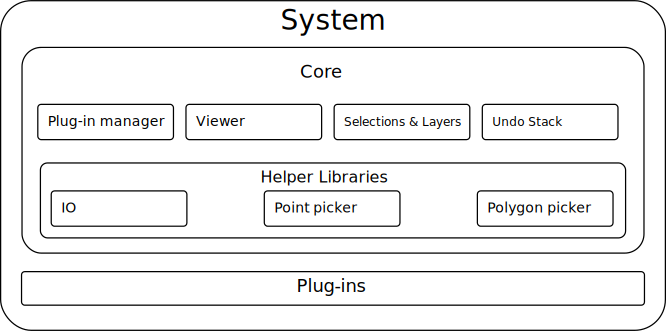
\includegraphics[width=.75\linewidth]{images/system}
  \caption[System architecture]{The system is implemented as a plug-in architecture. The user interface and state management is handled by the core system. Segmentation and other tools that manipulate the system state are loaded into the system as plug-ins.}
  \label{fig:system}
\end{figure}

\todo{Explain what is going on in captions}
\todo{Have algorithms everywhere}
\todo{System boot up in an algorithm}

\todo{Explain dependency graph and meta data}
\todo{Cross platform is useful for the comunity ast large, mention it as, plugins and compilation steps are non trivial, however that is not the main focus, provid emore detail in apendix, because it is peripheral}

The system core implements the functionality needed to view range images, manage range images, keep track of segmentations and load plug-ins. Some additional functionality that could be moved to plug-ins are also resident in the core system. This includes basic file import and helper functions for common UI problems.

\subsection{IO}

The system is currently limited to dealing with range images that with 3D coordinates and intensity values. Importing Cyclone PTX range images is built into of core system. PTX is an ASCII based interchange format created by Leica. The file format may contain multiple range images with 3D coordinates, intensity and RGB values. The file header also contains a 4x4 matrix that represents the registration transformation in addition to the scan grid dimensions \cite{Leica}. Following the header is the point data arranged in ordered in column major order. The format contains all the scan data including non returned points as that are represented as 0 0 0 for the XYZ coordinate.

Because a large number of points are typically not returned, they are discarded when loading a PTX file into the system. This reduces memory consumption and simplifies 3D rendering and manipulation. A separate data structure is kept that maps returned points back to their position in the scan grid. This insures that operations that rely on a point's position in the original scan grid, such as 2d rendering and normal computation, can still be performed. It also means that the PTX file can be saved in its original format.

The system makes use of PCL (Point Cloud Library) \cite{Rusu2011} data structures. This allows us to use many popular point cloud algorithms without implementing them from scratch.

\subsection{Segments} \label{sec:segments}

The core system need to keep track subsets of points identified by segmentation plug-ins. The data structures used in this book keeping task require some careful consideration. Our review of tools in existing systems allow us to gather some requirements.

Interactive tools such as a lasso or brush tool require that points be added or removed from a selection real time. Representing a selection as an array of indices would require an $O(n)$ operation for adding or removing points. If we instead represent a selection as an array of boolean values that are mapped to points, a selection can be modified in constant time. This representation however has the disadvantage of only allowing binary segmentations. One way of overcoming this limitation is to create additional boolean arrays for new segmentations. This solution is however not very efficient. The memory requirements each additional segmentation, would increase as factor proportional to the point cloud size.

This problem can be overcome if we only allow a single selection to be edited in real time. Selections not being manipulated can thus be saved in less performant but more compact data structures. As is common in many editors, we shall refer to these saved selections as layers.

To keep track of many layers we need the representation to be space efficient. If we assign an integer to every layer we wish to represent we could keep track of $2^{32}$ layers assuming layers are mutually exclusive. Without this assumption we would be limited to 32 layers. This 2nd solution has the nice property of supporting efficient set operations. Unions can be computable in $O(n)$ by performing a binary OR on each integer with a bitmask including all the layers in question. Intersection can be achieved by using a binary AND and subtractions can be achieved via XOR.

Set operations are useful for making existing tools more powerful by combining results. For example, if we had a tool that could isolate trees and another tool that could find leaves, we could isolate bare trees by subtracting the leaf result from the tree result. Performing set operations on unordered lists of indices would be prohibitively expensive. Keeping lists of indices sorted is another option but it would add overhead.

If we instead revert to assigning integer labels to points, and represent layers as points that are labeled with a given set of integers, we can achieve near constant time set operations while supporting a large amount of layers.

\begin{figure}[ht]
	\centering
	\includegraphics[width=0.45\textwidth]{images/layers1}
	\caption[Initial label state]{ Initially all points are labeled with `0' which is never assigned to a layer. \label{fig:layer1}}
\end{figure}

\begin{figure}[ht]
	\begin{minipage}[b]{\linewidth}
		\centering
		\includegraphics[width=0.45\textwidth]{images/layers2}
	\end{minipage}
	\\\\
	\begin{minipage}[b]{0.49\linewidth}
		\hfill
		\begin{tabular}[b]{|l|l|l|l|}
			\hline
			Layer & Label set \\
			\hline
			\textcolor{red}{red}       & 1 \\
			\hline
		\end{tabular}
	\end{minipage}
	\hspace{0.5cm}
	\begin{minipage}[b]{0.5\linewidth}
		\begin{tabular}[b]{|l|l|l|l|}
			\hline
			Label & Layer set \\
			\hline
			1       & \textcolor{red}{red} \\
			\hline
		\end{tabular}
		\hfill
	\end{minipage}
	\caption[Label state after creation of the first layer.]{ After the first layer is created the associated points are labeled with `1'. The label is associated with the red layer. \label{fig:3-layer2}}
\end{figure}

To illustrate the solution we developed, picture the labels associated with a set of points. We initially assign 0 to all points which we designate as being the state in which a point is not associated with any layers (see figure~\ref{fig:3-layer2}). If we wish to create a layer, we need to change the label of the points that belong to this layer. In our example we assign 1 to the points in our new red layer (see figure~\ref{fig:3-layer2}). The new label now has to be associated with the label set of the red layer. We thus add 1 to the label set.


\begin{figure}[ht]
	\begin{minipage}[b]{\linewidth}
		\centering
		\includegraphics[width=0.45\textwidth]{images/layers3}
	\end{minipage}
	\\\\
	\begin{minipage}[b]{0.49\linewidth}
		\hfill
		\begin{tabular}[b]{|l|l|l|l|}
			\hline
			Layer & Label set \\
			\hline
			\textcolor{red}{red}       & 1 \\
			\textcolor{green}{green}       & 2 \\
			\hline
		\end{tabular}
	\end{minipage}
	\hspace{0.5cm}
	\begin{minipage}[b]{0.5\linewidth}
		\begin{tabular}[b]{|l|l|l|l|}
			\hline
			Label & Layer set \\
			\hline
			1       & \textcolor{red}{red} \\
			2       & \textcolor{green}{green} \\
			\hline
		\end{tabular}
		\hfill
	\end{minipage}
	\caption[Two non overlapping layers]{ The creation of a second layer that does not overlap with others results in the creation of a new label which is assigned to the layer. \label{fig:3-layer3}}
\end{figure}

To add an additional non overlapping layer we follow the same process. First a new label is generated (2 in this example) and the points in the layer are labeled with it. The new label is then added to the label set of the new green layer (see figure~\ref{fig:3-layer3}.



\begin{figure}[ht]
	\begin{minipage}[b]{\linewidth}
		\centering
		\includegraphics[width=0.45\textwidth]{images/layers4}
	\end{minipage}
	\\\\
	\begin{minipage}[b]{0.46\linewidth}
		\hfill
		\begin{tabular}[b]{|l|l|l|l|}
			\hline
			Layer & Label set \\
			\hline
			\textcolor{red}{red}       & 1, 4 \\
			\textcolor{green}{green}       & 2 \\
			\textcolor{blue}{blue}       & 3, 4 \\
			\hline
		\end{tabular}
	\end{minipage}
	\hspace{0.5cm}
	\begin{minipage}[b]{0.5\linewidth}
		\begin{tabular}[b]{|l|l|l|l|}
			\hline
			Label & Layer set \\
			\hline
			1       & \textcolor{red}{red} \\
			2       & \textcolor{green}{green} \\
			3       & \textcolor{blue}{blue} \\
			4       & \textcolor{blue}{blue}, \textcolor{red}{red} \\
			\hline
		\end{tabular}
		\hfill
	\end{minipage}
	\caption[Three layers with one overlap]{Creating a layer that overlaps with others results in overlapping points be assigned a new label which is assigned to both layers.\label{fig:3-layer4}}
\end{figure}

Overlapping layers are more interesting. In figure~\ref{fig:3-layer4} we create a new blue layer that overlaps with the red layer. It is clear that we cannot follow the same procedure, as assigning a new integer label to the points in the blue segment would remove the overlapping points from the red layer. We solve this problem by creating two new labels. First we assign 3 to the points that do not overlap with the red layer. This label is then added to the blue layer's label set. The overlapping points are given the label 4. This label is then added to the label set of both the red and blue label. The blue and red layer now have a label in common.

Set operations can now be achieved by simply adding and removing labels from layers without accessing individual point labels. The number of labels that we can create is dependent on the number of layer intersections.

In the worst case scenario is each newly created layer overlaps with ever other layer. In this case the number of bits allocated for the label will be the maximum number of layers. Our 16 bit implementation therefore be limited to 16 layers. If no overlaps occur, 65536 layers could be created. The number of layers one an accommodate is equivalent to $2^b/e$ where $b$ is the number of bits used for a label and $e$ is the expected number of intersections for each newly created layer.

% TODO multiple clouds

\subsection{Undo}
Selections and layers encode the work performed by a user. We therefore need to allow users to undo actions that modify these data structures. Undo can be achieved via two software patterns; namely the command pattern or the memento pattern \cite{Gamma1995}. The memento pattern saves the state of the system before an action is applied. Undo can be achieved after an action is performed by restoring the original state. The command pattern encapsulates all information needed to perform some action in an object. The object can then be used to apply or undo some action.

The selection and layer states in our system can be large. The memento pattern could quickly exhaust memory resources when a large range image is loaded. Consider a brush selection tool. Such a tool may be dragged across the screen and issue multiple selection commands in quick succession. Each command would require a copy of the selection state of all the points in a range image. It is unlikely that a large amount states could be stored in this way.

The command pattern lets one keep track of changes far more efficiently. Only the information required to apply and undo action needs to be recorded. For the case of selections, we need only to save the newly selected points. When using the command pattern a series of selections need not consume unnecessary memory. 

In our system, we use the QT5 which fortunately provides much of the scaffolding needed to implement the command pattern. To implement custom commands the QUndoCommand class needs to be subclassed. The constructor of a custom command should be provided with all the information required to execute and undo a command. The redo and undo methods of a command are used to execute and rollback actions. Commands are managed by an instance of QUndoStack. Pushing a command to a QUndoStack invokes the redo method which results in the command being executed. Popping from a QUndoStack results in the undo method of the last command being invoked. QUndoCommands can also be merged. In the example of a brush tool one may create 100's of commands depending on how how long the action lasts. To undo 100's of commands for a single stroke would be tedious. Merging allows us to combine multiple commands into a single command.

In our system we provide five types of commands for manipulating selections and layers. There is a single select command that lets one select and deselect points. Layers can be created via two commands. The first lets one specify the indices in a point cloud that constitutes the layer and the second lets one specify a new layer in terms of labels in existing layers. There is also a layer delete command.

Plug-ins can only manipulate layers and selections via the specified commands which makes all actions reversible. 

\subsection{Rendering}
Our system uses OpenGL 3.3 to render both a 2D and 3D view of a loaded range image. During rendering range scans along with layer and selection data is copied into GPU memory (see \autoref{table:gpulayout}). All changes to the system state is kept synchronized with the GPU. No level of detail techniques are applied which limits our system to loading scans that can fit into GPU memory.

\begin{table}[ht]
	\begin{center}
	\begin{tabular}{|l|l|l|l|}
	\hline
	Index & X,Y,Z,I (float{[}4{]}) & Label buffer (uint16) & Selection mask (uint8)\\
	\hline
	0     & 0.8, 1.2, 0.2, 0.9 & 0                     & 10000000               \\
	1     & 0.7, 0.5, 0.8, 0.3 & 2                     & 10000000               \\
	2     & 4.3, 0.5, 1.7, 0.9 & 2                     & 10000000               \\
	3     & 0.6, 1.8, 0.1, 0.6 & 1                     & 01000000               \\
	4     & 0.9, 0.5, 0.8, 0.5 & 2                     & 01000000               \\
	5     & 0.1, 0.4, 3.2, 0.9 & 3                     & 01000000               \\
	6     & 2.2, 0.5, 0.3, 0.2 & 5                     & 00000000               \\
	7     & 1.0, 0.9, 0.1, 0.5 & 4                     & 00000000               \\
	\vdots     & \vdots & \vdots  & \vdots             \\
	\hline
	\end{tabular}
	\end{center}
	\caption[GPU buffer layout]{Three buffers are created on the GPU to render point clouds with layers. This comprises a buffer to hold the 3D coordinates and intensity value of each point, a buffer that maps labels to points, and a buffer to represent selections.}
	\label{table:gpulayout}
\end{table}


A 3D rendering is achieved by simply loading the points along with their intensity values onto the GPU and outputting the intensity value after camera transformations have been applied. The 2D rendering requires that mapping of points to the original scan grid is also loaded. In the original scan grid is then rendered via an orthogonal projection to the view port. The color value for a point in the grid is the intensity value of the point which it references or black if the point was not returned. 

Selections and layers are rendered by coloring the grayscale intensity values for points in the range image. The selection state of a point can be represented with a single bit. However, a byte is the smallest attribute data type that one can reference in a GLSL shader. This means in the selection buffer we will waste 7 bits for every point. Multiple selections proved to be useful in some segmentation plug-ins, it was thus decided that instead of wasting the bits, up to 8 selections will be supported via a selection mask.

To render selections the GLSL shader was modified so that each bit in the selection would map to a fixed colour. During rendering the shader will iterate over each bit in the selection mask to determine the average colour of the selections. This colour is then multiplied with the intensity value associated with the point.

\begin{table}[ht]
	\begin{center}
	\begin{tabular}{|l|l|l|l|}
	\hline
	Layer  name & Color    & Visible & Labels \\
	\hline
	grass       & \#009900 & true & 0, 2, 4      \\
	walls       & \#0000FF & true & 0, 3  \\
	tree        & \#00FF00 & false & 2, 3   \\
	\vdots     & \vdots & \vdots   & \vdots          \\
	\hline
	\end{tabular}
	\end{center}
	\caption[Layer data structure]{Label colours are precomputed averaging the colours of the layers associated with each.}
	\label{table:layers}
\end{table}

Rendering layers is a more involved process. The number of layers and associated colours are not fixed. Layers can also be toggled as invisible (see \autoref{table:layers}). To achieve alpha blending of intersecting colours we precompute the colour associated with each label (see section \ref{sec:segments}). Each label can be associated with one or more layers and each layer is assigned a colour. To compute the colour associated with a label we compute the average colour of all the visible layers associated with it. The result is a lookup table as shown in \autoref{table:colorlookup}. The lookup table is copied into a buffer texture that is used by the shader to find the blended label colour associated with each point. Changing layer colours or toggling a layer invisible only requires that the lookup tabel be recomputed and loaded to a GPU.


\begin{table}[ht]
	\begin{center}
	\begin{tabular}{|l|l|l|}
	\hline
	Label & Color  \\
	\hline
	0       & walls.color \\
	1       & grass.color \\
	3       & mix(walls.color, tree.color)	\\
	4       & grass.color	\\
	\vdots     & \vdots      \\
	\hline
	\end{tabular}
	\end{center}
	\caption{Label color lookup table}
	\label{table:colorlookup}
\end{table}

\subsection{Navigation}
In the \autoref{chapter:background} it was noted that navigating a point cloud or range image is an important part of the segmentation task. It was argued that when working with 3D environments as opposed to 3D objects, it may be more natural to use a 1st person navigation rather than a trackball. In our system the first person camera is the primary mode of navigation. The user can use the arrow keys or WASD keys to move forward or laterally. Q and E can be used to move up and down. The left mouse button can be clicked to look around and the right mouse button can be clicked to rotate the cloud around it's axis.

\todo{Footnote needs to start at 0}

\begin{figure}[ht]
  \centering
  \includegraphics[width=.5\linewidth]{images/head}
  \caption{Yaw, pitch, and roll axis of the camera. \protect\footnotemark[\value{footnote}]}
  \label{fig:head}
\end{figure}
\footnotetext{Source: \url{http://www.mdpi.com/1424-8220/13/11/15549/htm}}

When people move around the physical world, gravity is an important orienting cue that allows one to determine a spacial frame of reference \cite{Jeffery2011}. In virtual 3D environments this cue does not exists which can disorient users when encountering unfamiliar camera orientations. People are most familiar with navigating horizontal planes. Flipping this plane upside down or on its side can result in such an unfamiliar frame of reference.

Keeping the camera in an upright position relative to the range image ground plane would eliminate unfamiliar reference frames. This would hover limit the camera rotation to left and right (yaw axis). It is also necessary to look up and down (pitch axis, see \autoref{fig:head}). Rotating the camera by 180 degrees around the pitch axis would however result in a disorientating upside down view. Some systems and games prevent this by limiting the yaw rotations to 90 in both directions relative to the ground plane. A user that wishes to look beyond 90 degrees up or down is then forced to turn around first which is arguably more tedious. This also does not prevent the camera from rotating the roll direction. A disorientating roll rotation can still achieved by looking down and then looking left. Preventing a disorientating roll effectively results in an artificial gimbal lock \cite{Hanson2007} despite using quaternions.

In our system we developed a way to mitigate the problem of accidental disorientating reference frames without restricting camera rotations. The user is allowed to freely rotate the camera around the yaw and pitch axis. Translating the camera however incrementally corrects the roll rotation to be level with the ground plane. The amount of incremental roll correction per unit of translation is dependent on the pitch angle relative to the ground plane as given by \autoref{eq:rollcorrect}.

\begin{equation} \label{eq:rollcorrect}
   rollCorrectionFactor(pitch) = \left\{
     \begin{array}{lr}
       1 - abs(pitch-\pi/2)/(\pi/2) & : pitch \le \pi/2\\
       0 & : pitch  > \pi/2
     \end{array}
   \right.
\end{equation}

Rotating beyond 45 degrees disables roll correction as it is likely that the user intended to be orient the camera in this way. If the user is disorientated, corrective actions will quickly enable roll correction that will reorientate the user. Failing this a keyboard shortcut can be used to reset the camera orientation and translate the camera back to the origin.

The 2D view allows the user to pan the range image by dragging it. Scaling can be achieved by scrolling the mouse wheel. When the mouse wheel is scrolled the image first translated to the mouse position, scaled, an then the translation is reversed. This has the effect of zooming towards the mouse pointer.

\todo{Mention: birds eye view, point size, exponential decay interpolation}

\subsection{Plug-ins}
Plug-ins can insert functionality into many parts of the system. Menu items and settings panels can easily be added to the system by exposing GUI objects. Plug-ins that need to render to the view port can do so by listening do draw events from the 3D or 2D view ports. Draw events references the state of the widget that can be used by plug-ins to interact with OpenGL. View port input can also be intercepted installing event filters on view port widgets.

In addition to access to system events and objects, plug-ins have access to helper functions for common tasks. The two main helper functions exposes 2D and 3D point picking functionality as well as a 2D and 3D polygon lasso tool.

\todo{We implemented plugins [enumerate], then say discussed in chapter X}

\todo{Geometric point picking vs render picking?}
\todo{Project IO?}
% \subsection{UI Helpers}

% \subsection{Selected plug-ins}
% Should plug-ins be discussed here?
% Are the lasso lasso and brush tools innovations?
% Normal visualization plug-in
% Project export plugin.

% \subsection{Implementation specifics}
% PCL, QT, OpenGL?

\section{Conclusion}

We created an open source, cross platform, range image segmentation framework with key innovations being user super efficient layers and roll corrected 3D navigation. In addition all layer an selection commands can be rolled back via a undo stack which is not the case in existing open source packages.







% The centerpiece of the UI is the view port that renders the range image.


% The system core implements a basic GUI that includes a viewer and navigation. 


% that can be dynamically loaded and unloaded at runtime


% We want fast selections and layers


% Cloud compare has no plugins thus is hard to extend. Meshlab has to layers which complicates teh workflow

% Test wether first person navigation is better than track ball?

% In order to address these stumbling blocks a new system was created. The system is focused primarily on point cloud segementation

%  soley on range image segmentation rathe The key requirements for a point cloud system is a range image viewer 


% In this chapter discuss the design and implementation of the framework that will be built upon in susequent chapters.

% \section{Requirements}
% The aim of this system is to combine and improve the best parts of existing point cloud editing systems in an open source framework focused on fast point cloud segmentation. To achieve this objective the following subgoals were determined.

% \subsection{Usability}
% To speed up the cleaning task it is important that the system interface makes the task as easy as posible. To achieve this familar concepts and components are borrowed from existing systems in order to minimise the learning curve. This includes an undo stack which is missing from open source systems.

% % Stop the camera from flipping

% \subsection{Multi scan support}
% Range images in a set need to overlap in order for ICP registration to work. This means that same objects or noise can be present in two or more range images. Removing the same points from two or more scans increases cleaning time. In loading two or more scans at time, duplicate points can be removed with in with one action and save time.

% \subsection{Pluggable}
% Our cleaning framework encompases only the core elements one need to view, navigate and represent segmentations in range images. The tools to perform range image segmentation will be implemented as seperate components. This seperation of concerns reduces complexity, simplifies development, and reduces compile time. Runtime reloading of plugins further speeds up developement time as reloading the system and associated state is not neccesary.

% \subsection{Open source}
% Our system will be released as opensource so that our results maybe reproduced and the framework may be used as a platform for future research.

% \subsection{Cross platform}
% In order to maximise our reach our system will work on both Microsft Windows and Linux.

% \subsection{Limitations}
% Packages such as Cloud Compare support the loading of large point clouds. We limit our system to range images that fit into memory. This can be overcome by using level of detail rendering techniques but is out of the scope for the current project.

% \subsection{Technology stack}
% Point cloud processing and 3D rendering generally requires efficieny use of system resources in order to achive maximum performance. As such lower level systems languages that compile to efficient binaries seems like the most sensible choice. In our case C++ was chosen, not only due to it's speed and efficiency but also because it is used by the most popular point cloud processing library \emph{Point Cloud Library (PCL)} \cite{Rusu2011}.

% PCL includes extendable point cloud datastructures that can be used with implementations of many popular point cloud algorithms. Basic UI components lets one capture basic interactions and view results. These components are by no means suffient to create a user friendly point cloud editing system but lets one tests one's algorithms. 



% \section{Core system}

% As with all other 3D point cloud packages, the centerpiece of our system is a 3D point cloud viewer. In addition to this we provide a 2D range scan view in addition.


% An additional 2D range image view is also included as it 


% Our goal is to achieve

% The system is designed provide the basic functionality to load and view range scans as well as group points into selections and layers. Additional functionality is provided via a plugin system that facilitates both interactive and batch segmentations. All actions should be undoable.




% Meshlab's point cloud editing support is somewhat limited due to the primary focus being mesh editing. Meshlab's extention framwork lets one create new tools but is quite limiting. 

% Meshlan


% Goals
% 	Usability
% 		Ensures improvements in more advance tools are not hamstrung by a bad interface
% 	Support editing multiple scans
% 		Pairwise editing is quicker and can disabiguate sparse points
% 	Plugin architecture
% 		Support for interactive and batch segementation tools
% 	Quick development cycle
% 		Recompiling a large codebase is debilitating
% 	Cross platform
% 		Zamani uses windows so it was neccesary
% 	Open source
% 		Create a good base for future work

% Limitations
% 	Supporting range images larger than system or GPU memory is out of this scope of this project. 

% Core system
% 	2D + 3D view
% 	Navigation
% 		Prevent fipping the 3D view upside down
% 		Accelerated navigation
% 	Segmetation workflow
% 		Selections
% 			Primary representation of segmentation
% 			Needs to support multiple scans
% 		Layers
% 			Store of segementations
% 			Supports combining results from multiple segmentations
% 			Set operations
% 				Union, intersect, subtract
% 	IO
% 		Save & load progress
% 		Export final cleaned scans to PTX

% 	Full undo

% Plugin architecture
% 	Dynamic reloading of tools
% 		Recompiling the system in its entirity and reloading the program and data can be time consuming
% 		Recompiling and reloading a plugin is much quicker
% 	Tools need to hook themselves into the core system
% 		Meshlab vs QTCreator
% 			Meshlab has plugin types that are limited
% 				IO, Filters, Rendering
% 			QTCreator makes no such distinction and is thus more flexible


% Implementation
% 	C++, PCL, QT, OpenGL
% 		Justify choices? To what extent?
% 		Should I justify why I coded by own system instead of using VTK?

% 	Selections & Layers
% 		(Section already written)

% 	Rendering
% 		Filter non returned points (less memory)
% 		Create index grid that references filtered scan

% 	Save file format
% 		JSON was bad to I created a custom format

% 	Navigation
% 		Custom camera that prevents flipping
% 		2d zooming & panning, zoom towards mouse

% 	Tools for plugins
% 		Point picker
% 			Ray casting vs selection buffer

% 		Lasso?
% 			Maybe discuss this in another chapter?
% 			Should I cover my retarded OpenCL implementation?


% Segmentation
% Segmentation
% 	Mid level computer vision problem
% 	Segmentation is a term used for a wide range of techniques which have the same goal
% 	Use features to group related points
% 	Groups can be constucted so that they are similar, colour or texture, and then sumarised
% 	The details of what the summary representation should be dependent on the task but there are general desirable features
% 	Higher level algorithms should not be overwelmed by it
% 	It should be in a form that higher level algorithms, such as recognition algorithms, can use

% Clustering
% 	Methods that focus on local relations between items.
% 	This approach allows us, for example, to assemble together clumps of pixels that look similar. Such clumps are commonly called regions

% 	A key feature of the human vision system is that context affects how things are perceived. The gestalt school of psychologists emphasized grouping as the key to understanding visual perception. Their work was characterized by attempts to write down a series of rules by which image elements would be associated together and interpreted as a group. They felt some factors predisposed a set of elements to be grouped. Thes factors are important because it is quite clear that the human vision system uses them in some way.

% 	Rules:
% 	- Proximity: Tokens that are nearby tend to be grouped.
% 	- Similarity: Similar tokens tend to be grouped together.
% 	- Common fate: Tokens that have coherent motion tend to be grouped together.
% 	- Common region: Tokens that lie inside the same closed region tend to be grouped together.
% 	- Parallelism: Parallel curves or tokens tend to be grouped together.
% 	- Closure: Tokens or curves that tend to lead to closed curves tend to be grouped together.
% 	- Symmetry: Curves that lead to symmetric groups are grouped together.
% 	- Continuity: Tokens that lead to continuous—as in joining up nicely, rather than in the formal sense—curves tend to be grouped.
% 	- Familiar configuration: Tokens that, when grouped, lead to a familiar object

% 	These rules can function fairly well as explanations, but they are insufficiently crisp to be regarded as forming an algorithm. Gestalt factors provide interesting hints, but should be seen as the consequences of a larger grouping process, rather than the process itself.


% Applications:
% 	Background subtraction, anything that doesnt look like a backgound is interesting
% 		Known background then subtract to see segments, some threshold aplied
% 		Bad if background changes (avarage bg over time)
% 		Bad if background colour matches object

% 	Interative segmentation:
% 		Need to cut out objects
% 		Too much work using every pixel

% 		Background foreground segmentation
% 			Assumptions: foreground is coherent, background maybe not

% 		Inteligent scissors
% 			Sketch curve close to boundry, moved closer usig gradient or boundry cues
% 			Snakes!

% 		Painting interface
% 			Paint pixels with foreground or background brush
% 			Used to produce an appearance model that is fed into a graph based segmenter

% 			Grab cut (cite this), draw box or paint foreground and background (GrabCut Interactive Foreground Extraction using Iterated Graph Cuts)

% 			Box yeilds an intial segmentation



%\chapter{Segmentation}
The goal of segmentation is to partition data into meaningful subsets. In heritage range images such groupings often include, but are not limited to: points representing vegetation, walls, people or scanner artifacts. Isolating these points can be extremely difficult and time consuming. Suitable segmentation techniques for heritage cleaning should speed up the process by reducing a user's workload while maintaining interactivity.

% Interactive batch jobs

\section{Performance}
A key metric for measuring the utility of a technique is the time it takes to achieve a segmentation result. The total segmentation time is the sum of durations associated with each action. The time to perform a segmentation can thus be reduced by either minimizing the time consumed by individual actions or reducing the number of actions.

Reduction in the time consumed by an for user actions can be achieved via a good user interface, as discussed in \ref{chapter:framework}.The number of actions required by a user can be reduced by delegating work to an algorithm. It is important for an effective algorithm to produce a result within a reasonable amount of time. If a user could achieve an equivalent result without the algorithm in less time, the technique adds no value.

For non-synthetic range images, it is unlikely that an algorithm will produce a perfect segmentation. It is thus expected that remedial action by a user will almost always be required. The final segmentation will thus be the total time required by each algorithm action and remedial user actions.

\begin{figure}[ht]
  \centering
  \includegraphics[width=1\linewidth]{images/walltree.png}
  \caption[Imperfect segmentation]{Example of a imperfect segmentation. The wall (red and green region) was targeted but the red and blue region were selected. In order the produce the correct wall segmentation, a user will need to deselect the blue region (false positive), and select the green region (false negative) } 
  \label{fig:imperfectseg}
\end{figure}

For example, if an automated tool for wall segmentation selected 95\% of the wall and part of a nearby tree, a complete segmentation will only be achieved once the remaining 5\% of the wall is selected and the tree points removed (see \autoref{fig:imperfectseg}). If a user could previously perform the segmentation in 2 minutes, the automated tool would only be effective if it could allow a user complete the task in less than 2 minutes. If the wall segmentation tool needs 30 seconds to isolate the wall and then requires and additional 30 seconds of user action to refine the result, the tool can be considered useful as it can reduce the segmentation time by 1 minute. If however, the accuracy of the result is such that an additional 2 minutes of user action is required to achieve the same result, the tool provides no advantage over the status quo. The same can be said if the processing time pushed the total time over the 2 minute mark.

A high accuracy technique can minimize the amount of subsequent remedial user action required following its use. It should, however, be noted that accuracy is not directly related to reduced effort. Consider a wall selection tool that selects 50\% of a target wall. If the tool selected hard to isolate points and the remaining points could easily be selected with a single user action, the total time could still be low. This wall selection tool would exhibit low accuracy but would still be effective.


\section{Evaluation}

\begin{figure}[ht]
  \centering
  \includegraphics[width=1\linewidth]{images/precision_recall.png}
  \caption[Precision and recall]{Precision and recall \protect\footnotemark } 
  \label{fig:precision_recall}
\end{figure}
\footnotetext{Adapted from: \url{https://en.wikipedia.org/wiki/Precision\_and\_recall}}

Segmentation algorithms are typically evaluated in terms of precision and recall \cite{Ponce2012}. Given a set of points we define a subset as our target. If an algorithm selects another subset, the selected points can be divided into true positives and false negatives. The remaining points are either false negatives or true negatives (see \autoref{fig:precision_recall}).

Precision is then defined as the number of true positives selected as fraction of the total number of selected points.

\begin{equation} \label{eq:precision}
	\text{precision}=\frac{|\{\text{target points}\}\cap\{\text{selected points}\}|}{|\{\text{selected points}\}|}
   % \right.
\end{equation}

Recall is defined as the number of true positives as a fraction of the targeted points.

\begin{equation} \label{eq:recall}
	\text{recall}=\frac{|\{\text{target points}\}\cap\{\text{selected points}\}|}{|\{\text{selected points}\}|}
   % \right.
\end{equation}

These two measures can be combined as an F-score that represents accuracy. The score can be interpreted as the weighted average of precision and recall.

\begin{equation} \label{eq:f1score}
	F_1 = 2 \cdot \frac{\mathrm{precision} \cdot \mathrm{recall}}{\mathrm{precision} + \mathrm{recall}}
   % \right.
\end{equation}

Our position is unique in that user efficiency instead of accuracy is our primary objective. Accuracy is still a good indicator of how useful related research is likely to be. Computational efficiency however is at least as important as it contributes to the total task time.

\section{Evaluation technique}
In order to evaluate how effective a segmentation method is we need to know how long it will take a user to produce a segmentation given the method and how long a user will take without it. User testing is however time consuming and expensive. Instead of user testing we choose to develop a technique to simulates a user's segmentation actions.

The technique requires reference segmentation which is used to compute a series of user actions to reproduce the result. The reference segmentation can be reproduced from the ground up or from a pre-existing segmentation. Associating a time value with each user action allows us to estimate the time required to reproduce a reference segmentation.

In a real world cleaning task, users may have access to a variety of tools that work best in certain situations. Determining when a simulated user should use one tool over another may be difficult. Settling on a single tool allows us to drastically reduce simulation complexity. We have found, at one organisation, that point cloud cleaning was performed with the use of only a polygon select tool. While this may not be ideal, it does boost the ecological validity of a simplified single tool simulation. For this reason our simulation uses a polygon select tool.

As previously discussed, a polygon lasso tool is not ideal in situations where a target cannot easily be isolated. In 3D, a user can view the target from a position that minimizes the number of false selections (see \autoref{fig:3dselect}). Finding such an ideal vantage point would add significant computational complexity to a simulation. Instead, our simulation computes polygon selections in 2D. This allows us to avoid false selections of points behind the target. It can however result in more false selections of surrounding points (see \autoref{fig:2dselect}).

\begin{figure}
\centering
\begin{subfigure}{.33\textwidth}
  \centering
  \includegraphics[height=6cm]{images/3dselect/1.png}
  \captionsetup{margin=5pt}
  \caption{This perspective makes it hard to avoid cable selection}
\end{subfigure}%
\begin{subfigure}{.33\textwidth}
  \centering
  \includegraphics[height=6cm]{images/3dselect/2.png}
  \captionsetup{margin=5pt}
  \caption{False selection can be avoided via a different perspective}
\end{subfigure}
\begin{subfigure}{.33\textwidth}
  \centering
  \includegraphics[height=6cm]{images/3dselect/3.png}
  \captionsetup{margin=5pt}
  \caption{False selection were not completely avoided and requires remedial action}
\end{subfigure}
\caption{3D polygon selection}\label{fig:3dselect}
\end{figure}


\begin{figure}
\centering
\begin{subfigure}{.3\textwidth}
  \centering
  \includegraphics[height=6cm]{images/2dselect/1.png}
  \caption{Polygon around target}
\end{subfigure}%
\begin{subfigure}{.3\textwidth}
  \centering
  \includegraphics[height=6cm]{images/2dselect/2.png}
  \caption{Resultant selection}
\end{subfigure}
\begin{subfigure}{.3\textwidth}
  \centering
  \includegraphics[height=6cm]{images/2dselect/3.png}
  \caption{False positives are identifiable from a different perspective}
\end{subfigure}
\caption{2D polygon selection}\label{fig:2dselect}
\end{figure}


The first step in emulating the polygon selection tool is to find groups of points, within the reference set, that the user is likely to target (see \autoref{fig:clusters}). A simple 2D euclidean clustering algorithm achieves this \cite{Rusu2009a}. The clustering algorithm uses KD-tree to grow a region as long as the next point is within a threshold distance of the last. The minimum size of a cluster also needs to be specified.

Given a cluster, the boundary is established by computing a concave hull \cite{Moreira2006} (see \autoref{fig:concavehull}). The algorithm used is a variation of the gift-wrapping convex hull algorithm \cite{Jarvis1973}. First, an extrema in the y or x axis is found. The K-nearest neighbours at the extrema are then computed. The first edge of the hull is created between the extrema and the neighbour that makes the biggest right hand turn relative to the extrema axis. The next point is selected in the same manner but the right hand turn is measured relative to the previous edge. Each edge, other than the starting edge, can only be visited once. When the starting point is reached again the hull is complete. The starting vertex can only be revisited after the 3rd iteration. This ensures that the algorithm does not terminate prematurely. The K that is chosen for the neighbour search affects how dense the hull is and how many outliers are excluded.

The computed hull around a cluster usually consist of a large number of boundary points. A human is unlikely to use as many points or be as precise. The number of points are reduced by applying a polygon simplification algorithm \cite{Ramer1972} (see \autoref{fig:simplification}). The simplification algorithm ensures that for any point P in between points A and B on the polygon, the distance to line AB from C will be greater than a given threshold. If this is not true the point is removed.

The simplification algorithm may shrink the hull and produce false negatives. The hull can, however, only shrink in proportion to the threshold selected for the simplification. To compensate for the reduced size the hull can be expanded proportionally outwards (see \autoref{fig:expand}). Each point in the hull is moved outwards along the 2D point normal. The adjustment needs to be such that the false positive are minimised.


\begin{figure}
\centering
\includegraphics[height=4cm]{images/evaltool/scan.png}
\caption[Clustering step]{Clustering the reference segmentation (black dots) into 2 clusters (green and blue dots)}\label{fig:clusters}
\end{figure}


\begin{figure}
\centering
\begin{subfigure}{.3\textwidth}
  \centering
  \includegraphics[height=3cm]{images/evaltool/tree1.png}
  \captionsetup{margin=5pt}
  \caption{Concave hull}
  \label{fig:concavehull}
\end{subfigure}%
\begin{subfigure}{.3\textwidth}
  \centering
  \includegraphics[height=3cm]{images/evaltool/tree2.png}
  \captionsetup{margin=5pt}
  \caption{Polygon simplification. This step can create false negatives (black and red dots)}
  \label{fig:simplification}
\end{subfigure}
\begin{subfigure}{.3\textwidth}
  \centering
  \includegraphics[height=3cm]{images/evaltool/tree3.png}
  \captionsetup{margin=5pt}
  \caption{Dilating the simplified hull. False negatives (red and white dots) can be added by this step}
  \label{fig:expand}
\end{subfigure}
\caption{Creating a realistic polygon around the first cluster}
\label{fig:polygoncluster}
\end{figure}



\begin{figure}
\centering
\begin{subfigure}{.3\textwidth}
  \centering
  \includegraphics[height=4cm]{images/evaltool/individual.png}
  \caption{Individual cluster selection}
  \label{fig:individualclusters}
\end{subfigure}%
\begin{subfigure}{.3\textwidth}
  \centering
  \includegraphics[height=4cm]{images/evaltool/goodselect.png}
  \caption{Multi cluster selection}
  \label{fig:multicluster}
\end{subfigure}%
\begin{subfigure}{.3\textwidth}
  \centering
  \includegraphics[height=4cm]{images/evaltool/badselect.png}
  \caption{Multi cluster selection results in a false positive}
  \label{fig:badmulticluster}
\end{subfigure}
\caption{Selecting multiple clusters}\label{multiselect}
\label{fig:test}
\end{figure}



The previous steps assume the user will select each cluster individually (see \autoref{fig:individualclusters}). This assumption does not always hold true. In a real world task, less effort may be required to select multiple clusters of points with a single polygon (see \autoref{fig:multicluster}). However, if the polygon around the clusters result in a false positive or negative selection (see \autoref{fig:badmulticluster}), further actions will be required to correct it. It therefore needs be determined whether the larger selection followed by remedial actions, or individual selections, are less less effortful.

After computing polygons for each cluster, we determine if multiple clusters can be selected with a single polygon. To do this each pair of polygons are merged by computing their combined convex hull \cite{Andrew1979}. We then check if the selection produced by the combined hull creates false selections in addition to those produced by the individual hulls. If the false selections are below a threshold the two hulls are replaced by the merged hull. These steps are repeated on all subsequent hull pairs. 

The steps described above will produce false selections. To improve accuracy, false positive and false negative points are clustered and the algorithm is repeated. Hulls associated with false negative points will be selected and those associated with false positive points will be deselected. This process can be repeated until a predetermined level of accuracy is reached. This is analogous to the refinement that takes place into real point cloud cleaning.

While each iteration may improve the accuracy of the segmentation, the extra simulated effort may not be worth the marginal increase in accuracy. An iteration can also produce as many false positives as the false negatives that were eliminated. The algorithm should thus terminate either when a set accuracy is reached, or the marginal improvement is not sufficient to justify the additional effort.

\begin{algorithm}
  \caption{Lasso tool simulation\label{alg:eval}}
  \begin{algorithmic}[1]
    \Let{$simplificationFactor$}{$5$}
    \Let{$falseSelectionCount$}{\Call{countFalseSelection}{$selection, target$}}
    \Let{$iterations$}{$0$}
    \While{$falseSelectionCount > threshold$ $\|$ $iterations <maxItterations$}
      \Let{$falsePositives$}{$selection - target$}
      \Let{$falseNegatives$}{$selection \cap target^c$}

      \Let{$fpClusters$}{\Call{Cluster}{$falsePositives$}}
      \Let{$fnClusters$}{\Call{Cluster}{$falsePegatives$}}

      \Let{$fpHulls$}{\Call{ConvexHull}{$fpClusters$}}
      \Let{$fnHulls$}{\Call{ConvexHull}{$fnClusters$}}

      \State\Call{Simplify}{$fpHulls, simplificationFactor$}
      \State\Call{Simplify}{$fnHulls, simplificationFactor$}

      \State\Call{Expand}{$fpHulls, simplificationFactor$}
      \State\Call{Expand}{$fnHulls, simplificationFactor$}

      \For{$ i \gets 0 \textrm{ to } fpHulls.length$} \Comment{Merge hulls}
        \For{$ j \gets i \textrm{ to } fpHulls.length$}
          \Let{$combined$}{\Call{Merge}{$fpHulls_i, fpHulls_j$}}
          \If{\Call{HasFalseSelection}{$combined, target$}}
            \Let{$fpHulls_i$}{$combined$}
            \State $fpHulls.remove(j)$
            \Let{$j$}{$j - 1$}
          \EndIf
        \EndFor
      \EndFor

      \For{$ i \gets 0 \textrm{ to } fnHulls.length$} \Comment{Merge hulls}
        \For{$ j \gets i \textrm{ to } fnHulls.length$}
          \Let{$combined$}{\Call{Merge}{$fnHulls_i, fnHulls_j$}}
          \If{\Call{HasFalseSelection}{$combined, target$}}
            \Let{$fnHulls_i$}{$combined$}
            \State $fnHulls.remove(j)$
            \Let{$j$}{$j - 1$}
          \EndIf
        \EndFor
      \EndFor

      \State\Call{Deselect}{$fphulls$}
      \State\Call{Select}{$fnhulls$}
      \Let{$itterations$}{$itterations + 1$}
      \Let{$falseSelectionCount$}{\Call{countFalseSelection}{$selection, target$}}
    \EndWhile


  \end{algorithmic}
\end{algorithm}

\todo{How is this determined}

\subsection{Metrics and ecological validity}
To estimate the time a user will take to reproduce a segmentation, we need to associate a time value with the placement of each vertex in a polygon. The overhead associated with starting and finalising each polygon also needs to be determined.

To correctly estimate the total segmentation time, the algorithm actions need to mirror user's polygon and vertex counts. We can modify the number of vertices in a polygon by setting the threshold of the polygon approximation algorithm. The number polygons constructed can be adjusted by modifying the termination condition.\todo{clarify}

Test data was collected by asking users to segment five objects of varying complexity in a pilot study of five users \cite{Mathematical1910}. Users were shown the reference segmentation before starting each scan and asked to obtain a similar level of detail. The time users took to invoke and finalise each polygon was recorded, as well as the number of points in each polygon and time to draw each polygon. The recall and precision for each segmentation was also recorded.

Results show that the system accurately mirrors the number of points real users use for their polygons.

% \section*{Test data}
% Isolated
% Interspersed
% Coherent


\section{Segmentation methods}

Segmentation algorithms include a variety of related methods with the same goal of grouping related data points. Points can be grouped either by considering local or global relations. These two organizing principles are not always mutually exclusive. Techniques that group points via local relations are called called clustering methods. The goal of such methods is to ensure grouped points are similar. As an example we may group together green points. The second set of techniques group points that share some global relationship. Points that lie on a plane may be grouped, not because of any local relationship, but because when seen as a whole the points represent a surface. These techniques are typically rely on a model.

\subsection{Features}\label{sec:features}

In order to group points we need a way of comparing them to each other or a model. Raw properties of the dataset such as 3D coordinates and intensity can be used. These properties are also called features. A feature vector is used to collect relevant measurements that describe a point. Raw scans contain lots of redundancies and noise data that can make it hard to effectively exploit.

Better data representation can be obtained through feature engineering or feature learning. The aim of both methods is to transform the raw data in a way that brings forward useful properties given task at hand. The difference is that feature engineering often relies on expert knowledge determine the transformation, where as feature learning aims to produce the transformation via learning techniques.

Features can not only used to describe points, but also groups of points. Hierarchical groupings can be used in this way to produce suitable level of abstraction for a given task. This is similar to the bottom up processing the human visual system performs on low level stimuli.


\subsection{Segmenting via clustering}

Clustering methods attempt to organise points into meaningful or useful assemblies. Depending on the task at hand, this may be sufficient to produce a meaningful segmentation. Often however, it is only a first step in a more elaborate process.

The first step in clustering a dataset is to select good features. One could use raw features or the result of preprocessing step. A distance metric then needs be selected that will be used as a pairwise similarity measure. The final step to applying a grouping algorithm that determines which points belong together.

\subsubsection*{Feature selection}

Selecting the right feature is critical in producing meaningful results. For example, when grouping points by colour, the selected the colour representation may affect the outcome. Red green blue (RGB), may produce different groupings when compared to Hue Value Saturation (HSV). Clustering with only colour information will lead points with a similar colour to all me part of one cluster. Including positional information in the feature vector will ensure that only points that are similar in colour and are close together is grouped.

Given a raw dataset one could generate a near inexhaustible number of features. Knowledge of the problem area may help one reduce the search space. Many domain specific features have been developed that help solve common problems. In 2D computer vision transformations exist that help identify edges \cite{Marcelja1980}, textures \cite{Hadjidemetriou} and other salient features \cite{Dalal}. In 3D range imaging similar descriptors have been engineered, such as Point Feature Histograms, that encodes local geometric information in a pose invariant manner, while being tolerant to noise and variation in sampling density \cite{Rusu}.  

Hand crafting features or even parametrising established features may require substantial effort. Learning algorithms allows one to discover features without expert knowledge or human effort. Features can be learned via supervised or unsupervised methods.

In supervised learning, a labelled training set used to create a classifier that maps unlabelled data to new features. Dictionary learning is one such instance. The idea is to map input points to weighted vector of dictionary elements \cite{Mairal2009}.

Unsupervised approaches do not require training sets. Instead the goal is to discover lower dimensional features in higher dimensional spaces. K-means clustering can be used in such a manner. The idea is to group data into k subsets. Point can then be represented by the k-dimensional vector representing the distance to the centroid of each of the k clusters \cite{Coates2012}.

What constitutes a good set of features ultimately depends on how well they performs as part of a task. A feature can be evaluated in isolation by correlating it with what labelled data. A good feature will be strongly correlated with important properties of the data data. Weak features can however also be useful when combined with other features. It is thus important to not only consider feature sin isolation.


% http://blog.datadive.net/selecting-good-features-part-i-univariate-selection/

% http://en.wikipedia.org/wiki/Feature\_learning


\subsubsection*{Distance metric}

A suitable distance metric should be a good indicator how similar two points are. Most clustering algorithms default to using a Euclidean distance metric \cite{Grabusts2011}. Euclidean distance is the square root of the sum of squared differences of each component in a feature vector. As result a large disparity for single component of a pair of feature vectors can have large effect on the metric. This may or may not be desirable. To mitigate this effect components of a feature vector is regularised so that each component has a similar range. Some components may be more important than other in which case it may be desirable to weigh them. Hand tuning of distance metrics may result in substantial effort. \citet{Xing2002} proposed an automated method capture people's common sense understanding of similarity.


\subsubsection*{Grouping methods}

Given a distance metric and feature set we can now apply a number of different grouping algorithms to our dataset. Clustering algorithms can loosely be categorised according to their cluster model.

\begin{figure}
\centering
\includegraphics[height=4cm]{images/hierarchical-clustering}
\caption[Hierarchical clustering]{Hierarchical clustering}\label{fig:dendrogram}
\end{figure}



Hierarchical clustering is based on the idea that data points that are close together in feature space should be grouped together. The process starts by considering each point to be a cluster of size one. The two clusters that are closest together are then combined into a new cluster. This process continues until all points form one cluster. This produces a tree of clusters called a dendrogram (see \autoref{fig:dendrogram}). A dendrogram can be created bottom up (agglomerative clustering), as described, or top down (divisive clustering) where a single cluster is recursively split. Each level in the dendrogram is marks the distance where two clusters merged. A number of clusters can be produced by setting an appropriate merge or split threshold. Hierarchical clustering has an advantage over other methods in that the number of clusters do not have to be predetermined. The algorithm however has a complexity of $O(n^3)$ which makes it inappropriate for all but small datasets.

\begin{figure}
\centering
\includegraphics[height=4cm]{images/kmeans}
\caption[Hierarchical clustering]{K-means clustering \protect\footnotemark}\label{fig:kmeans}
\end{figure}

\footnotetext{Source: \url{https://pafnuty.wordpress.com/2013/08/14/non-convex-sets-with-k-means-and-hierarchical-clustering/}}


K-means clustering is computationally less expensive than hierarchical clustering. The disadvantage is that the number of clusters needs to be known upfront. An inappropriate choice can lead to bad results. The basic idea is to select K centroids and create groups by associating each input point with one of the centroids. The aim is to assign points to groups such that the average distance from a point to it's centroid is minimized. Because this optimisation is NP-hard, implementations use heuristics to compute approximate solutions \cite{Ponce2012}. K-means clustering is also limited in that it cannot deal with non convex sets (see \autoref{fig:kmeans}).

The high cost of agglomerative clustering can be overcome by first over segmenting a dataset with k-means clustering. The if the number of clusters produced k-means clustering is small enough the $O(n^3)$ cost of hierarchical clustering may be low enough to be practical.


Density-based clustering is another class of algorithms in which clusters are defined by areas of high point density. Mean-shift clustering \cite{Comaniciu2002} is an iterative approach where a kernel function is used to compute the centroid over an area of influence. For each iteration kernel is moved in the direction of the centroid until a local maxima is reached. Each point that converges to the same local maxima is assigned to a cluster. Mean shift can find arbitrary shaped clusters and the number of clusters do not have to be specified before hand. DBSCAN \cite{Ester1996} has similar properties but only requires a single pass and is thus computationally less expensive. Density based clustering algorithms pose a problem when applied to range images as the point density is non uniform. 


\begin{figure}
\centering
\includegraphics[height=10cm]{images/cluster-comparison}
\caption[Clustering algorithms]{Comparing different clustering algorithms on toy datasets \protect\footnotemark}\label{fig:compareclustering}
\end{figure}

\footnotetext{Adapted from: \url{http://scikit-learn.org/stable/auto_examples/cluster/plot_cluster_comparison.html}}

\subsection{Segmentation as graph partitioning}

When applying clustering algorithms to vision segmentation problems, some level of object coherence is expected. One is therefore likely to compare points that are close together. Clustering therefore naturally lends itself to being represented as a graph partitioning problem where neighbouring points are locally connected via edges that represent similarity.


\citet{Felzenszwalb2004} demonstrates this graph theoretic approach in the segmentation of 2D images. Each pixel is represented by a vertex and edge weights of neighbouring pixels indicate their dissimilarity. Each pixel is initially a cluster of one and the algorithm iterates over the edges in non decreasing order. If an edge spans two clusters and the edge weight is less than the internal difference between the clusters, the two are merged. The internal difference of a cluster is the largest edge weight inside it plus a biasing term gives small clusters higher weights.

Graph cuts are useful when a segmentation can be expressed as an energy minimisation problem. The idea is that each graph edge has a cost associated with it. Two vertices that are not part of the original graph are designated as the source and the sink (see \autoref{fig:graphcut}). Existing vertices are connected the source and the sink via weighted edges. The aim is then to separate the graph into two sub graphs containing the source and the sink by cutting the edges with the minimum cost. Segmentation tasks are typically formulated such some object is associated with the sink, and another object is associated with the source. The edges connecting to the source or sink indicates how strongly the vertex is associated with the source and sink. The weights between image vertices are set such that similar vertices are weighted heavily. The optimal cut is likely to include edges with lower weights. Because finding the minimum cost cut is the same as finding the maximum flow between the source and the sink, the optimisation can be performed in $O(VE^2)$ \cite{Edmonds1972}.


\begin{figure}
\centering
\includegraphics[height=10cm]{images/graphcut}
\caption[Graph cut]{Each pixel in the image is connected to it's neighbours, the source, and the sink. The aim of the graph cut is to remove the set of edges with the minimum weight, such that two sub graphs are created that contain the source and the sink. \protect\footnotemark}\label{fig:graphcut}
\end{figure}

\footnotetext{Source: \url{http://www.ondrej-danek.net/en/research}}


\citet{Boykov2001b} showed how graph cuts can be effectively used to perform foreground background segmentation on raster images by labelling part of the foreground and background. \citet{Boykov2001a} generalised this method to N-dimensional images and demonstrated how it can be used interactively to improve segmentation results in 2D raster images. Naive graph cuts sometimes do not perform well because the optimisation to cuts of smallest possible part of the graph in order to minimise the cut. So solve this issue \citet{Malik2000} proposed Normalised cuts in which the cost of the cut takes into account the affinity of the two graphs that would be created by a cut. That is to ensure that the two created graphs have have strong internal edge weights and weak edge weights between each other.



\subsection{Segmentation as classification}

% Grab cut

% forming image regions (sometimes use as the exclusive meaning of segmentation)
% 	decompose an image into regions that have roughly coherent color and texture.
% 	Typically, the shape of these regions isn’t particularly important, but the coherence is important
% 	regions allow us to deal with larger areas of an image without considering each element. (summary representation)
% 	super pixels can expose structure in images



% Clustering can be applied to points or groups of points

\subsection{Model driven segmentation}

Not all segmentation tasks can be performed by grouping of elements that are similar. It is often necessary to combine elements that conform to some model instead of, or in addition to clustering.

The Hough transform is a well known instance of when parametric model needs to be considered in order to segment create a segmentation that conforms to a model \cite{Ballard1981}. The Hough transform can however be prohibitively expensive to compute for all but the simplest models.

Model fitting is typically approached by trying to minimize an error function that indicates how well data conforms. Mean least squares simple way to achieve this. If we were trying to fit a plane to some data set, computing the squared error term for each point's deviation from plane. This would give us an indication of how well the plane fits the data. Given is information we could iteratively make adjustments to the plane's orientation and position in until a good fit is achieved.

This process would be significantly faster if we had a good original estimate of where the plane was. Pre-computing useful features such as corners or other key points can help register a model to good initial estimate. Clustering the data into higher level abstractions also reduces the computational workload \todo{cite that heritage paper}.

In practise data is noisy and outliers can make otherwise well behaved data not fit the model. RANSAC \cite{Fischler1981} is a fitting procedure that takes this variability into account. First one needs to determine what is the minimum number of points ($n$) one need to represent the abstraction one needs to identify. For a line $n$ would be 2, and for a plane or a sphere $n$ would be 3. Some threshold distance $t$ then needs to picked. Points further than $t$ will not be considered as fitting the model. Finally it needs to be decided how many samples is needed to confirm a model and how many outliers will be tolerated. The procedure is then to sample $n$ points at random and fit the model to them. Points are then selected at random until the model can be confirmed or rejected according to the predetermined parameters.

\todo{Tree models of canopies}
\todo{Kinect example}
\todo{Active contour model?}
\todo{Gaussian mixture model?}



\subsection{Applications}

Points that represent vegetation is undoubtedly some of the hardest classes of points to classify. Some of the most successful approaches to isolating vegetation have used scanners capable of full wave form analysis \cite{Reitberger2009, Elseberg2011}. These special scanners can detect multiple echos per emitted laser pulse. Multiple laser echos occur when more than one surface reflects the pulse. When scanning vegetation multiple echo's occur frequently because of their structure.\\

\citet{Elseberg2011} demonstrated that full wave form analysis can be used to achieve 95\% accuracy when segmenting trees from terrestrial scans on a university campus. It is unclear whether individual or merged ranges scans are used. The algorithm first projects all points to the ground plane and creates an occupancy grid. Points in in each cell are then classified as vegetation or not according to the pulse characteristics in the cell. The segments are then refined with a two pass clustering algorithm that ensures connected components have the same label. To further refine the segmentation the ratio of the two largest principle components of clusters were used distinguish trees from planar structures. A second approach to refining the clusters was adapted from \citet{Reitberger2009}. It computed a point density histogram along the vertical plane of clusters. The histogram was used with a support vector machine (SVM) to identify tree clusters. This approach produced less accurate results on the campus dataset.\\

The datasets in this research were not produced with full wave form scanners. The structure of vegetation will however produce variation in a range scan depth map. It is worth investigating whether this variation could potentially be exploited in a similar manner.\\

% multiple pulses
% principle components
% histograms of clusters

\citet{Reitberger2009} used the shape of the histogram to determine the height of a tree crowns in a clusters. Given the height of tree crown the number of stems could be estimated and an N-cut algorithm could be applied to separate trees in a cluster. This researched focused on segmenting individual trees in aerial scans of forests. In this instance a full wave form scanners was not essential to the segmentation algorithm but rather useful because it penetrates the forest canopy and allow trees below the canopy to be imaged. Terrestrial scanners do not need to penetrate canopies. The technique however, uses watershed segmentation on a projected point cloud to construct initial clusters. This approach is unlikely to be satisfactory when buildings, people and other objects are present. Other vegetation segmentation techniques are similarly inapplicable because the focus are in scenes with only vegetation \cite{Haugerud2001} or the targeted data sets are low density aerial scans \cite{Charaniya2004}.\\

% n-cuts

\citet{Barnea2012} describes an generic approach to extracting objects from color range scans that achieves 99\% accuracy on the test data. Problems with non uniform density is overcome by treating the scan as a panoramic image. Small holes in the image are interpolated from neighboring areas and a preset values are assigned to missing background data and larger regions. Mean shift clustering is used iteratively on individual image channels. The largest segment is removed and then the image is segmented again until no more segments above the threshold remain. Features derived from the range (sum of derivatives, sum of absolute derivatives, cornerness), color (HSV and Luv color space) and intensity (cornerness) are used in this process. The extracted segments are then classified as tree or non tree by a kNN classifier. The kNN classifier is trained with an example set using the same features. The segmentation is further refined using the a graph cut.\\

The color channels in the test data does not seem to contribute much discriminative power. A similar approach could thus be useful for our datasets that have no color information. Learning features means the no domain knowledge is required and the approach generalizes to other objects. Producing test data and training a classifier is however problematic in an interactive scenario. The upfront work required to produce test data may not be worthwhile if the resulting classifier only works on data similar to the training set. The kNN algorithm also poses problems as the optimal number of neighbors and the search radius needs to be determined. Features also need to be scaled correctly in order for the kNN classifier to work. The overhead of a classifier may not be necessary in an interactive environment if the user can easily select and remove unwanted segments.\\



% Canny edge detection is a simple instance where the image features are computed with a series of filters and then subsequently grouped in accordance with an edge model \cite{Canny1986}.

% Model must account for variation, hard to define

% Hough transform
% Ransacs
% Machine learning


% Features
% 	What is a good feature
% 	How to design or pick a good feature?
% 		Something that correlates with what you are trying to segment?
% 		Only evaluated as part of a learning/segmentation/clustering algorithm?
% Clusters
% Interactive segmentation
% Machine learning
% 	Deep nets
% 		Learn features via unsupervised
% 	SVG
% 	Random forests
% 	Graph optimasation

% Existing systems
% 	Range images
% 	Point clouds
% 	Aerial scans
% 	What features are used?
% 	Clustering
% 	Machine learning
% 	Level of accuracy
% 	Interactive?
% 	Assumptions?


% %!TEX root = thesis.tex
\chapter{Literature review} \label{ch:lit}

\section{Previous work}
Point cloud cleaning is a interactive segmentation problem. Segmentation is by no means a new problem.

\subsection{Taxonomy}
\begin{itemize}
	\item Interactive/Automated
	\item Information: 2D/2.5D/3D/nD, color, multi-sample, intensity
	\item Resolution: High, Medium, Low
	\item Features: Texture, FPFH, Normals, ...
	\item Target: trees, ground, walls, people, generic
	\item Parameters: Low, Medium, High
\end{itemize}


\subsection{Image segmentation}
	Scans are simply a depth maps so 2D image techniques should be investigated
	\subsection{Image gradients}
	\subsection{Edge detection}
	\subsection{Blob extraction}
	\subsection{Contour extraction}

\subsection{Laser scan segmentation}
	\subsection{Point features}
		\subsubsection{Normals}
			Basic building block for other features
			\begin{itemize}
			\item Ways of performing normal estimation
			\item Neighbour search
				\begin{itemize}
				\item KD Trees
				\item Scan grid
				\end{itemize}
			\item Cost vs Quality
			\item Dealing with noise
			\item Used with machine learning algorithms
			\end{itemize}
				
		\subsubsection{Fast point feature histograms (FPFH)}
			\begin{itemize}
			\item Good discrimination for primitive geometric objects
			\item Costly to calculate
			\end{itemize}
			
		\subsubsection{Principle components}
			\begin{itemize}					
			\item Good for finding edges and planes
			\item Solves part of the inverse problem
			\end{itemize}
			

	\subsection{Region growing}
		\begin{itemize}
		\item Grow neighbourhood from seed point
		\item Add neighbour if it satisfies some similarity criteria
		\item Point feature can be used to determine similarity
		\end{itemize}

	\subsection{K-means clustering}
		Problems with non uniform density

	\subsection{Graph cuts}
		\begin{itemize}
		\item Binary classification
		\item Encode point similarity edges
		\item Shown to work well with arbitrary objects
		\item Results are parameter depended
		\end{itemize}

	\subsection{Machine learning}
		\begin{itemize}
		\item Used in navigation \& aerial scans
		\item Support vector machines
		\item Markov models
		\item Conditional random fields
		\item Requires training
		\end{itemize}
		
	% \subsection{Evaluation of literature}
	% 	\begin{itemize}
	% 	\item FPFH seems to discriminate well for primitive geometry. Might be a useful feature to use in tree classification.
	% 	\item Machine learning has been used to classify vegetation. It however requires training and classified datasets are rare. Possibility to train a classifier on the on scans in the application. Unpredictable accuracy.
	% 	\item Graph cuts have been shown be effective for automated object classification. Augmented with more edge information accuracy may be improved with minimal user interaction.
	% 	\end{itemize}

\section{Evaluation techniques}
\begin{itemize}
	\item What was used in previous work and would it be suitable in this instance?
\end{itemize}
	
% \section{User interaction}
% 	\begin{itemize}
% 		\item Level of interactivity expected?
% 		\item Characteristics of interfaces?
% 		\item Basic expected functionality?
% 		\item Suitable evaluation techniques
% 	\end{itemize}
% %!TEX root = thesis.tex
\chapter{Design} \label{ch3}

\section{Design Goals}


\todo[inline, color=green!40]{Todo}


% % % What is needed to evaluate this question
% % % research design
% %!TEX root = thesis.tex
\chapter{Implementation} \label{ch3}

\section{s1}

\subsection{s2}
% % % Technical details of implementation
% %!TEX root = thesis.tex
\chapter{Evaluation} \label{ch:eval}

In this chapter the performance of roll correction and example based segmentation is evaluated.

\section{Roll correction}

We hypothesise that roll correction reduces disorentation that in turn leads to faster navigation of environments. To test this hypothesis three targets were chosen in a laser scan of a fort environment. Users were then tasked to navigate to these positions from two non upright starting positions. The goal is to navigate to the target position in an upright orientation as quickly as possible.

A plugin was created to set up a starting position and orientation, as well as determine how long it takes a user to reach the right orientation and target position.

[image here of targets, starting position and plugin]

Users were tasked to nagivate to each location with roll correction on and off. Each condition was repeared twice per location so learning effects could be counterbalanced. The order of the tasks was either be abba or baab where a designates roll correction being on and b designates roll correction being turned off. Reduce learning effects users were primed via 2 test runs under each condition.

The locations were mixed together to minimise learning effects.

Users were sampled from the general university population. Users had varying degrees of experience with computers. As users act as their own baselines the variation in skill level is not a concern. To test whether roll correction improves navigation speed a one tailed repeated measures t-test is used.

Prime on CccC
Group A aBAbAbaB
Group B bABaBabA

\section{Depth sensitivity of brush tool}

Segemnt heinz with depth sensitivity
Segment heinz without depth senistivity

Group A: AbbA
Group B: bAAb

\section{Example based segmentation}

As discussed earlier, the effectiveness of example based segmentation is based on whether the a user can perform a segmentation task in less time with the help of the segmentation method than without it. With this in mind a segmentation task was created in which a user was tasked to reproduce a ground truth segmentation within a predetermined accuracy level (f-score).

A repeated measures design was used. Users were asked to reproduce a segmentation using basic segmentation tools (lasso, brush, plane selection). In the first condition the user was asked to reproduce a segmentation from scratch. In the second condition the user was presented with a pre-existing segmentation as a starting point. The pre-existing segmentation was the result of example based segmentation. (provide pictures of the pre-existing segmentation)

Three different segmentations were used. In the first scene the target is a tree that is growing over a house. The second scene a spade, wheelbarrow, and some pots has to be isolated. In the third scene a person has to be removed.

To reduce learning effects the user is primed by via three segmentation tasks in which the 3 basic tools tool are introduced. Order effects are reduced by counterbalancing the order in which the task two condition are presented for each task.

A plugin was created present the user with the current accuracy every second for the set segmentation target. It also records accuracy over time.

Results are compared via a repeated measure one tailed ttest. The time taken to produce the presegmentation is added to the result of the condition where the user started with it. This accounts for the approximate time the user whould have taken if he or she use the tool him or herself. The pre-segmentation however lets us remove a source of variance.

Use lasso to segment heinz for 1min
Use wall tool to segment wall for 1min

Segment tree from wall
Segement objects of the ground

Group A: AaaABbbB
Group B: BbbBAaaB


\section{Noise filtering}

Show how the radius factor thinggie helps

\section{Test the different paremeters in the tree}


\section{Testing goals}

Do proper priming
Undo & redo
Selections, deselections
How to navigate, wasd qe

Don't have the green selection be present on the preselection tests


!!!!!!!!!!!!!!!!!!
Next, set up the spreadsheet to record results, users should be assigned to group 1 or 2 which have different counterbalance profiles.

The proceedures should also be outlined so that its clear that in instructions where given in the same way. Use a psych textbook or something to write this up in the correct structure.

Address:
proceedure constant
fatugue - short tasks
mention pilot study
CHECK TTEST ASSUMPTIONS!

!!!!!!!!!!!!!


test if the roll correction helps
test if the automated segmentation helps


explicit research question
express assumptions in operational definitions of terms

test whether roll correction is better than ordinary navigation
(btw how did we determine the roll correction factor)

what population do we want to generalise?
all people?

sampling bias?

need to eliminate meaurement error - repeated measures
learning effects - prime the user so the difference does not reflect a learning effect, (latin square) randomise order, keep experiment short to limit learning
fatigue - keep experiment short

because the effect is likely to vary between people, we need multiple people to make sure the effect is consistent?


number of needed participants is determined by error size / variance

we could get one sample of experts, or measure relative speed up?

between-participants design. In such a design, each person sees one—
and only one

control for order effects

not between participants because we would need a large sample to reduce error, or get a very homogenous sample

yes, latin square

An
experiment where each participant sees every condition (i.e., every level of ev-
ery factor) is, naturally enough, referred to as a within-participant design


2.2 The Elements of an Experiment

check that a all the assumptions for the t-test etc is true


For example, we can and do get better at pointing.
Most evidence suggests, however, that B (x) will remain constant (or nearly so) for short periods of time. (2.1.3)

Since the effects in most perception experiments are rather
large, a very rough estimate of e w is sufficient to be able to get a decent idea of
B (x). Thus, five to twenty repetitions are usually sufficient. Fewer than five rep-
etitions do not usually provide enough information to define e w . Using more
than twenty repetitions in a short period of time without specific precautions is likely to lead to fatigue, overlearning, or other masking effects (for more on
what those precautions are, please refer to a text on advanced experimental de-
sign such as Falmagne, 1985; Gescheider, 1997; Maxwell and Delaney, 1990).(2.1.3)

It should be men-
tioned that there are methods for determining the number of repetitions that
one needs, and some of these methods are discussed in Chapter 12. The use of
multiple measurements or repetitions of a given situation in an experiment is
called a repeated measures design.

2.1.6 Change versus Transformation

\begin{itemize}
\item User testing feedback on tools
\item Expert option

\item Correlate feature with segmentation
\item Calculate recall and recognition

\end{itemize}
% % Evaluation procedure
% % First tried experts in participatory design
% % Its bad so we try technology probe (put this in design)
% % How participants were recruited
% % How bias was avoided

% %!TEX root = thesis.tex
\chapter{Conclusion} \label{ch:conclusion}


\section{Future work}


\bibliography{thesis}
\bibliographystyle{plainnat}

\end{document}
